\documentclass{article}

% Language setting
% Replace `english' with e.g. `spanish' to change the document language
\usepackage[english]{babel}

% Set page size and margins
% Replace `letterpaper' with `a4paper' for UK/EU standard size
\usepackage[letterpaper,top=2cm,bottom=2cm,left=3cm,right=3cm,marginparwidth=1.75cm]{geometry}
\usepackage{CJKutf8}
% Useful packages
\usepackage{amsmath}
\usepackage{graphicx}
\usepackage{setspace}
\usepackage{float}
\usepackage{subfigure}
\usepackage[section]{placeins}
\usepackage[colorlinks=true, allcolors=blue]{hyperref}
\usepackage[export]{adjustbox}
\usepackage{array}

\author{B10209040 陳彥倫}

\begin{document}
\thispagestyle{empty}
\hfill {\scshape \large Statistics with Meteorological Applications, Spring 2024} \hfill {\scshape P1}
\smallskip
\hrule
\begin{CJK*}{UTF8}{bsmi}
\bigskip
\bigskip
\bigskip

\centerline{\huge \textbf {HW5}}
\bigskip
\centerline{\textbf {B10209040 陳彥倫}}


\section*{1.}
    \begin{spacing}{2.5}
        \begin{large}
            虛無假設:2000年的平均降雨量與氣候平均無差異。\\
            對立假設:2000年的平均降雨量與氣候平均有差異。
        \end{large}
    \end{spacing}

\section*{2.}
    \begin{spacing}{2.5}
        \begin{large}
            虛無假設:近15年(1999-2013)的全球平均溫度不大於上世紀初15年(1901-1915)的平均溫度。\\
            對立假設:近15年(1999-2013)的全球平均溫度大於上世紀初15年(1901-1915)的平均溫度。\\
            將顯著水準設為0.05,意即Z=1.645,並按公式解出要滿足顯著大於之$\overline{X}$的門檻約為12.42°C
            而年平均處理後的近15年平均溫度約為12.08°C,顯示近15年的全球平均溫度並未顯著大於上世紀初15年的平均溫度。
        \end{large}
    \end{spacing}

\section*{3.}
    \begin{spacing}{2.5}
        \begin{large}
            The observational time evolution of the canonical BSISO (left, CB) and northward-propagating 
            dipole-type BSISO (right, DB) from pentad −4 to pentad +4. Shading denotes the anomalous OLR 
            (W m−2), and vectors show the 850-hPa wind anomalies (m s−1; not shown when wind speed is less 
            than 0.5 m s−1). The green stippling denotes the regions at the 5\% significance level for composite 
            OLR anomalies.
        \end{large}
    \end{spacing}
        
\newpage
\thispagestyle{empty}
\hfill {\scshape \large Statistics with Meteorological Applications, Spring 2024} \hfill {\scshape P2}
\smallskip
\hrule    
\bigskip
\bigskip

\begin{figure}[h]
    \centering
    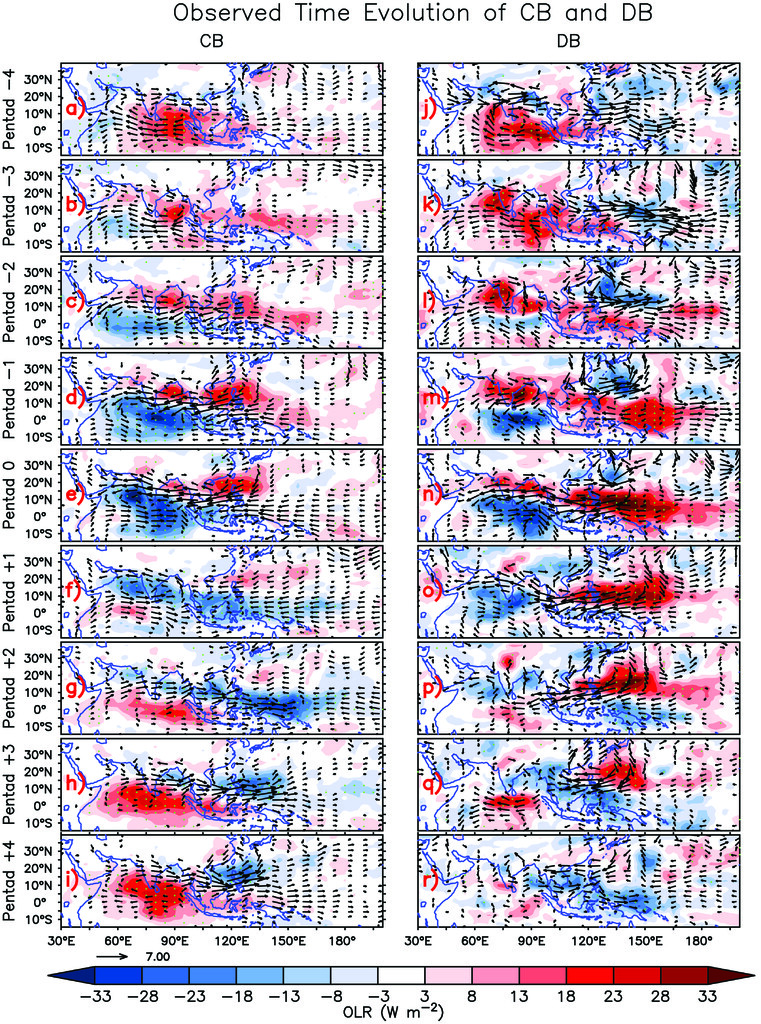
\includegraphics[width=12cm]{full-JCLI-D-23-0601.1-f2.jpg}
    \caption{Source: Baoqiang, X., Bin, W., Guosen, C., and Thomas, L. D.(2024).Prediction of Diverse 
    Boreal Summer Intraseasonal Oscillation in the GFDL SPEAR Model. \emph{Journal of Climate}.}
\end{figure}

\section*{}
    \begin{spacing}{2.5}
        \begin{large}
            \textbf{Remark:\\}
            圖中顯示了兩種類型的北半球夏季季內震盪(BSISO):標準型BSISO(CB)、Northward dipole BSISO(DB)於觀測
            時間內的演化情形。此圖亦包含了該範圍外射長波輻射強
        \end{large}
    \end{spacing}

\newpage
\thispagestyle{empty}
\hfill {\scshape \large Statistics with Meteorological Applications, Spring 2024} \hfill {\scshape P3}
\smallskip
\hrule    
\bigskip
\bigskip

\section*{}
    \begin{spacing}{2.5}
        \begin{large}
            度及風向風速。而此處利用5\%的顯著水準來判斷OLR的異常區域,但似乎沒有明確說明虛無假設及對立假設。
        \end{large}
    \end{spacing}


\end{CJK*}
\end{document}